\documentclass{article}

% content/resources/templates/preamble.tex
\usepackage[margin=0.6in]{geometry}
\author{Milav Dabgar}
\usepackage{amsmath,amssymb,amsthm}
\usepackage{booktabs}
\usepackage{multirow}
\usepackage{xcolor}
\usepackage{tcolorbox}
\tcbuselibrary{breakable,skins}
\usepackage[colorlinks=true,linkcolor=blue]{hyperref}
\usepackage{titlesec}
\usepackage{enumitem}
\usepackage{tikz}
\usepackage{pgfplots}
\usepackage{circuitikz}
\usepackage[version=4]{mhchem}
\usepackage{longtable}
\usepackage{array}
\usepackage{float}
\usepackage{caption}
\usepackage{listings}

\lstset{
  basicstyle=\small\ttfamily,
  breaklines=true,
  breakatwhitespace=false,
  postbreak=\mbox{\textcolor{red}{$\hookrightarrow$}\space},
  float=false,
  numbers=left,
  numberstyle=\tiny\color{gray},
  numbersep=10pt,
  xleftmargin=2em,
  keywordstyle=\color{blue},
  commentstyle=\color{green!60!black},
  stringstyle=\color{purple},
  backgroundcolor=\color{gray!5},
  showstringspaces=false,
  tabsize=2,
  captionpos=b,
  keepspaces=true,
  columns=flexible
}

\pgfplotsset{compat=1.18}
\usetikzlibrary{shapes,arrows,positioning,calc,patterns,decorations.pathmorphing,decorations.markings,arrows.meta}

% Color scheme
\definecolor{headcolor}{RGB}{0,102,204}
\definecolor{keycolor}{RGB}{220,20,60}
\definecolor{solutioncolor}{RGB}{34,139,34}
\definecolor{mnemoniccolor}{RGB}{148,0,211}
\definecolor{codecolor}{RGB}{0,0,100}

% Spacing
\setlength{\parskip}{3pt}
\setlist[itemize]{nosep}
\setlist[enumerate]{nosep}

% Title formatting
\titleformat{\section}{\Large\bfseries\color{headcolor}}{\thesection}{1em}{}
\titleformat{\subsection}{\large\bfseries\color{headcolor}}{\thesubsection}{1em}{}

% Pandoc tightlist compatibility
\providecommand{\tightlist}{%
  \setlength{\itemsep}{0pt}\setlength{\parskip}{0pt}}

% Pandoc longtable compatibility
\newcounter{none}
\def\thenone{}


% content/resources/templates/english-boxes.tex

% Custom environments
\newtcolorbox{solutionbox}{
 breakable,
 enhanced,
 colback=solutioncolor!5!white,
 colframe=solutioncolor!75!black,
 fonttitle=\bfseries,
 title=Solution
}

\newtcolorbox{solutionboxnobreak}{
 colback=solutioncolor!5!white,
 colframe=solutioncolor!75!black,
 fonttitle=\bfseries,
 title=Solution
}

\newtcolorbox{keyformula}{
 breakable,
 enhanced,
 colback=keycolor!5!white,
 colframe=keycolor!75!black,
 fonttitle=\bfseries,
 title=Key Formula
}

\newtcolorbox{mnemonicboxenv}{
 breakable,
 enhanced,
 colback=mnemoniccolor!5!white,
 colframe=mnemoniccolor!75!black,
 fonttitle=\bfseries,
 title=Mnemonic
}

\newcommand{\mnemonicbox}[1]{%
  \begin{mnemonicboxenv}
    #1
  \end{mnemonicboxenv}
}


% Custom commands for GTU solutions
% This file defines semantic commands for consistent formatting

% Question command with automatic formatting
\newcommand{\question}[2]{%
  \section*{Question #1}%
  \textbf{#2}%
}

% OR question variant
\newcommand{\questionor}[2]{%
  \section*{Question #1 OR}%
  \textbf{#2}%
}

% Proper table environment with caption
\newenvironment{answertable}[1]{%
  \begin{table}[htbp]
  \centering
  \caption{#1}
}{%
  \end{table}
}

% Proper figure environment for diagrams
\newenvironment{answerdiagram}[1]{%
  \begin{figure}[htbp]
  \centering
  \caption{#1}
}{%
  \end{figure}
}

% Semantic markup for key terms
\newcommand{\keyword}[1]{\textbf{#1}}
\newcommand{\code}[1]{\texttt{#1}}
\newcommand{\classname}[1]{\texttt{#1}}
\newcommand{\methodname}[1]{\texttt{#1}}

% Proper quotation marks
\newcommand{\mnemonic}[1]{``#1''}


\title{Fundamentals of Electronics (DI01000051) - Summer-2025 Solution}
\date{June 12, 2025}

\begin{document}
\maketitle

% ========================================
% QUESTION 1(a): Circuit Drawing (3 marks)
% Demonstrates: CircuiTikZ for electronic circuits, smart quotes, ~100 words
% ========================================

\questionmarks{1(a)}{3}{Draw a simple RC (Resistor-Capacitor) low-pass filter circuit.}

\begin{solutionbox}
An \keyword{RC low-pass filter} is a passive electronic circuit that allows ``low-frequency signals'' to pass while attenuating `high-frequency signals'. It consists of a \keyword{resistor} (R) and \keyword{capacitor} (C) connected in series.

\textbf{Circuit Diagram:}
\begin{center}
\begin{circuitikz}[scale=1.2]
    % Input terminals
    \draw (0,0) to[short, o-] (0.5,0);
    \node[left] at (0,0) {$V_{in}$};
    
    % Resistor
    \draw (0.5,0) to[R, l=$R$] (3,0);
    
    % Capacitor to ground
    \draw (3,0) to[short, -*] (4,0);
    \draw (4,0) to[C, l=$C$] (4,-2);
    \draw (4,-2) to[short, -o] (4,-2.5);
    \node[ground] at (4,-2.5) {};
    
    % Output terminals
    \draw (4,0) to[short, -o] (5,0);
    \node[right] at (5,0) {$V_{out}$};
\end{circuitikz}
\captionof{figure}{RC Low-Pass Filter Circuit}
\end{center}

\textbf{Key Characteristics:}
\begin{itemize}
    \item \keyword{Cutoff Frequency}: $f_c = \frac{1}{2\pi RC}$ (frequency at which output is 70.7\% of input)
    \item \keyword{Low Frequencies}: Pass through with minimal attenuation
    \item \keyword{High Frequencies}: Blocked by capacitor acting as low impedance to ground
\end{itemize}
\end{solutionbox}

\begin{mnemonicbox}
\mnemonic{RC-LP: Resistor-Capacitor blocks High, passes Low}
\end{mnemonicbox}

% ========================================
% QUESTION 1(b): Mathematics Calculation (4 marks)
% Demonstrates: Math equations, step-by-step calculation, inline \code{}, ~150 words
% ========================================

\questionmarks{1(b)}{4}{Calculate the cutoff frequency of an RC low-pass filter with $R = 1.5\,k\Omega$ and $C = 100\,nF$. Also find the output voltage if input is 10V at cutoff frequency.}

\begin{solutionbox}
\textbf{Given Data:}
\begin{itemize}
    \item Resistance: $R = 1.5\,k\Omega = 1500\,\Omega$
    \item Capacitance: $C = 100\,nF = 100 \times 10^{-9}\,F$
    \item Input Voltage: $V_{in} = 10\,V$
\end{itemize}

\textbf{Step 1: Calculate Cutoff Frequency}
The \keyword{cutoff frequency} formula for RC low-pass filter is:
$$f_c = \frac{1}{2\pi RC}$$

Substituting values:
$$f_c = \frac{1}{2\pi \times 1500 \times 100 \times 10^{-9}}$$
$$f_c = \frac{1}{2\pi \times 1.5 \times 10^{-4}}$$
$$f_c = \frac{1}{9.42 \times 10^{-4}} = 1061.57\,Hz \approx 1.06\,kHz$$

\textbf{Step 2: Calculate Output Voltage at Cutoff}
At cutoff frequency, output voltage is \keyword{0.707 times} (or $\frac{1}{\sqrt{2}}$) the input voltage:
$$V_{out} = 0.707 \times V_{in} = 0.707 \times 10 = 7.07\,V$$

\textbf{Results:}
\begin{itemize}
    \item \keyword{Cutoff Frequency}: $f_c = 1.06\,kHz$
    \item \keyword{Output Voltage}: $V_{out} = 7.07\,V$ at cutoff
    \item \keyword{Attenuation}: $-3\,dB$ at cutoff frequency
    \item \keyword{Phase Shift}: $-45^\circ$ at cutoff frequency
\end{itemize}
\end{solutionbox}

\begin{mnemonicbox}
\mnemonic{RC-Formula: fc = 1/(2$\pi$ RC), Vout = 0.707 Vin at fc}
\end{mnemonicbox}

% ========================================
% QUESTION 1(c): Comparison Table (7 marks)
% Demonstrates: Comprehensive comparison, \tabulary{} with caption at TOP, ~250 words
% ========================================

\questionmarks{1(c)}{7}{Compare active and passive electronic components with suitable examples.}

\begin{solutionbox}
Electronic components are classified into \keyword{active} and \keyword{passive} categories based on their ability to control or amplify electrical energy.

\begin{center}
\captionof{table}{Active vs Passive Components Comparison}
\begin{tabulary}{\linewidth}{|L|L|L|}
\hline
\textbf{Characteristic} & \textbf{Active Components} & \textbf{Passive Components} \\ \hline
Energy Source & Require external power source & Do not require external power \\ \hline
Control Ability & Can control/amplify current flow & Cannot amplify, only regulate \\ \hline
Directionality & Usually unidirectional & Bidirectional \\ \hline
Power Gain & Provide power gain ($>1$) & Power gain is always $\leq 1$ \\ \hline
Examples & Transistors (BJT, FET), Diodes (LED, Zener), ICs (Op-Amp, 555 Timer), SCR & Resistors, Capacitors, Inductors, Transformers \\ \hline
Function & Amplification, switching, oscillation, rectification & Resistance, capacitance, inductance, filtering \\ \hline
Linearity & Can be linear or non-linear & Generally linear \\ \hline
\end{tabulary}
\end{center}

\textbf{Active Components in Detail:}
\begin{itemize}
    \item \keyword{Transistors}: Used for amplification and switching. BJT uses current control, FET uses voltage control.
    \item \keyword{Diodes}: Allow current in one direction. LED emits light, Zener regulates voltage.
    \item \keyword{ICs}: Integrated circuits like \code{555 timer} (oscillator), op-amps (amplifier).
    \item \keyword{Power Requirement}: All active components need DC bias/supply to operate.
\end{itemize}

\textbf{Passive Components in Detail:}
\begin{itemize}
    \item \keyword{Resistors}: Oppose current flow, dissipate power as heat. Value in $\Omega$.
    \item \keyword{Capacitors}: Store energy in electric field. Value in Farads (F), blocks DC, passes AC.
    \item \keyword{Inductors}: Store energy in magnetic field. Value in Henry (H), opposes AC changes.
    \item \keyword{Transformers}: Transfer energy between circuits via magnetic coupling.
\end{itemize}

\textbf{Key Distinction:}
The fundamental difference is that active components can ``inject power'' into a circuit (amplification), while passive components can only ``absorb or store'' energy, never increase it.
\end{solutionbox}

\begin{mnemonicbox}
\mnemonic{ACTIVE = Amplify, Control, Transform; PASSIVE = Resist, Store, Filter}
\end{mnemonicbox}

% ========================================
% QUESTION 1(c OR): Alternative Question (7 marks)
% Demonstrates: OR question format, TikZ diagram with gtu styles, lstlisting, ~250 words
% ========================================

\questionmarks{1(c OR)}{7}{Draw and explain the working of a half-wave rectifier circuit with input and output waveforms.}

\begin{solutionbox}
A \keyword{half-wave rectifier} converts AC voltage to pulsating DC by allowing only one half-cycle (positive or negative) of the input AC waveform to pass through.

\textbf{Circuit Diagram:}
\begin{center}
\begin{circuitikz}[scale=1.2]
    % AC Source
    \draw (0,0) to[sV, l=$V_{in}$] (0,2);
    \draw (0,2) to[short] (2,2);
    
    % Diode
    \draw (2,2) to[D*, l=$D$] (4,2);
    
    % Load Resistor
    \draw (4,2) to[short] (5,2);
    \draw (5,2) to[R, l=$R_L$] (5,0);
    \draw (5,0) to[short] (0,0);
    
    % Output voltage measurement
    \draw (4.5,2) to[short, *-] (4.5,2.5);
    \node at (4.5,2.7) {$V_{out}$};
    \draw (4.5,0) to[short, *-] (4.5,-0.5);
    \node[ground] at (4.5,-0.5) {};
\end{circuitikz}
\captionof{figure}{Half-Wave Rectifier Circuit}
\end{center}

\textbf{Working Principle:}
\begin{enumerate}
    \item \keyword{Positive Half-Cycle}: When input AC is positive, diode is forward-biased (conducts). Current flows through load resistor $R_L$, producing output voltage.
    \item \keyword{Negative Half-Cycle}: When input AC is negative, diode is reverse-biased (blocks). No current flows, output voltage is zero.
    \item \keyword{Result}: Only positive half-cycles appear at output, creating pulsating DC.
\end{enumerate}

\textbf{Waveform Representation:}
\begin{center}
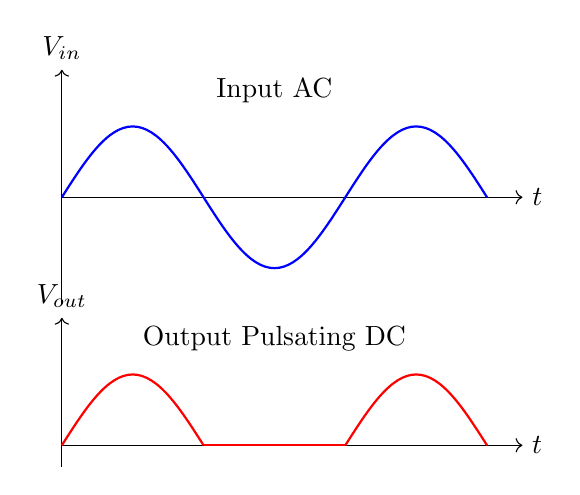
\begin{tikzpicture}[scale=0.9]
    % Input waveform
    \draw[->] (0,0) -- (6.5,0) node[right] {$t$};
    \draw[->] (0,-1.5) -- (0,1.8) node[above] {$V_{in}$};
    \draw[thick, blue] (0,0) sin (1,1) cos (2,0) sin (3,-1) cos (4,0) sin (5,1) cos (6,0);
    \node at (3,1.5) {Input AC};
    
    % Output waveform
    \begin{scope}[yshift=-3.5cm]
        \draw[->] (0,0) -- (6.5,0) node[right] {$t$};
        \draw[->] (0,-0.3) -- (0,1.8) node[above] {$V_{out}$};
        \draw[thick, red] (0,0) sin (1,1) cos (2,0);
        \draw[thick, red] (2,0) -- (4,0);
        \draw[thick, red] (4,0) sin (5,1) cos (6,0);
        \node at (3,1.5) {Output Pulsating DC};
    \end{scope}
\end{tikzpicture}
\captionof{figure}{Input and Output Waveforms}
\end{center}

\textbf{Key Parameters:}
\begin{itemize}
    \item \keyword{Efficiency}: $\eta = 40.6\%$ (theoretical maximum)
    \item \keyword{Ripple Factor}: $r = 1.21$ (high ripple content)
    \item \keyword{Peak Inverse Voltage (PIV)}: $PIV = V_m$ (maximum reverse voltage across diode)
    \item \keyword{DC Output}: $V_{DC} = \frac{V_m}{\pi} = 0.318 V_m$ where $V_m$ is peak AC voltage
\end{itemize}

\textbf{Applications:}
Half-wave rectifiers are used in low-power applications like battery charging, signal demodulation, and voltage multipliers. They are \textit{not suitable} for high-power applications due to poor efficiency.
\end{solutionbox}

\begin{mnemonicbox}
\mnemonic{HWR: Half-Wave = Half output, 40.6\% efficiency, PIV = Vm}
\end{mnemonicbox}

\end{document}
